\documentclass{article}

% set font encoding for PDFLaTeX or XeLaTeX
\usepackage{ifxetex}
\ifxetex
  \usepackage{fontspec}
\else
  \usepackage[T1]{fontenc}
  \usepackage[utf8]{inputenc}
  \usepackage{lmodern}
  \usepackage{graphicx}
  \usepackage{float}
\fi

% used in maketitle
\title{
        \begin{center}
        
\includegraphics[width=8cm]{Unison.png}
        \end{center}
        \newline
        Evaluación 1.- Análisis de las mareas y salinidad en el Manglar El Sargento.}
        
\author{Jose Burruel Martinez}
\date{8 de Marzo del 2018}

% Enable SageTeX to run SageMath code right inside this LaTeX file.
% documentation: http://mirrors.ctan.org/macros/latex/contrib/sagetex/sagetexpackage.pdf
% \usepackage{sagetex}

\begin{document}
\maketitle .

\section{Introducción}
Se tiene una estación de monitoreo de variables atmosféricas, CO2, radiación solar, nivel de agua y salinidad en el \textit{Manglar El Sargento}, en una bahía en la costa frente a la parte norte de la Isla Tiburón.
Nos interesa explorar los datos de Febrero de 2018 de nivel de mar, salinidad y temperatura del agua. Se proporcionan los datos de cada 15 minutos en formato CSV. 

Lo que se hará es un analisis extensivo de estos datos para graficar y observar la correlación que tienen unos con los otros.

\section{Pasos a seguir}
\subsection{Limpiar los datos}
Lo primero que se tiene que hacer es, ya que se descargaron los datos proporcionados por el profesor, verificar que la estructura de ellos esté \textit{limpia}, lo que significa que tenemos que ver si estan acomodados en columnas para poder trabajar dichos datos así como lo hemos estado haciendo anteriormente. Si no están así, se deberán abrir los archivos en \textit{emacs} para poder modificarlos. 

Los datos se ven de la siguiente manera:
\begin{figure}[H]
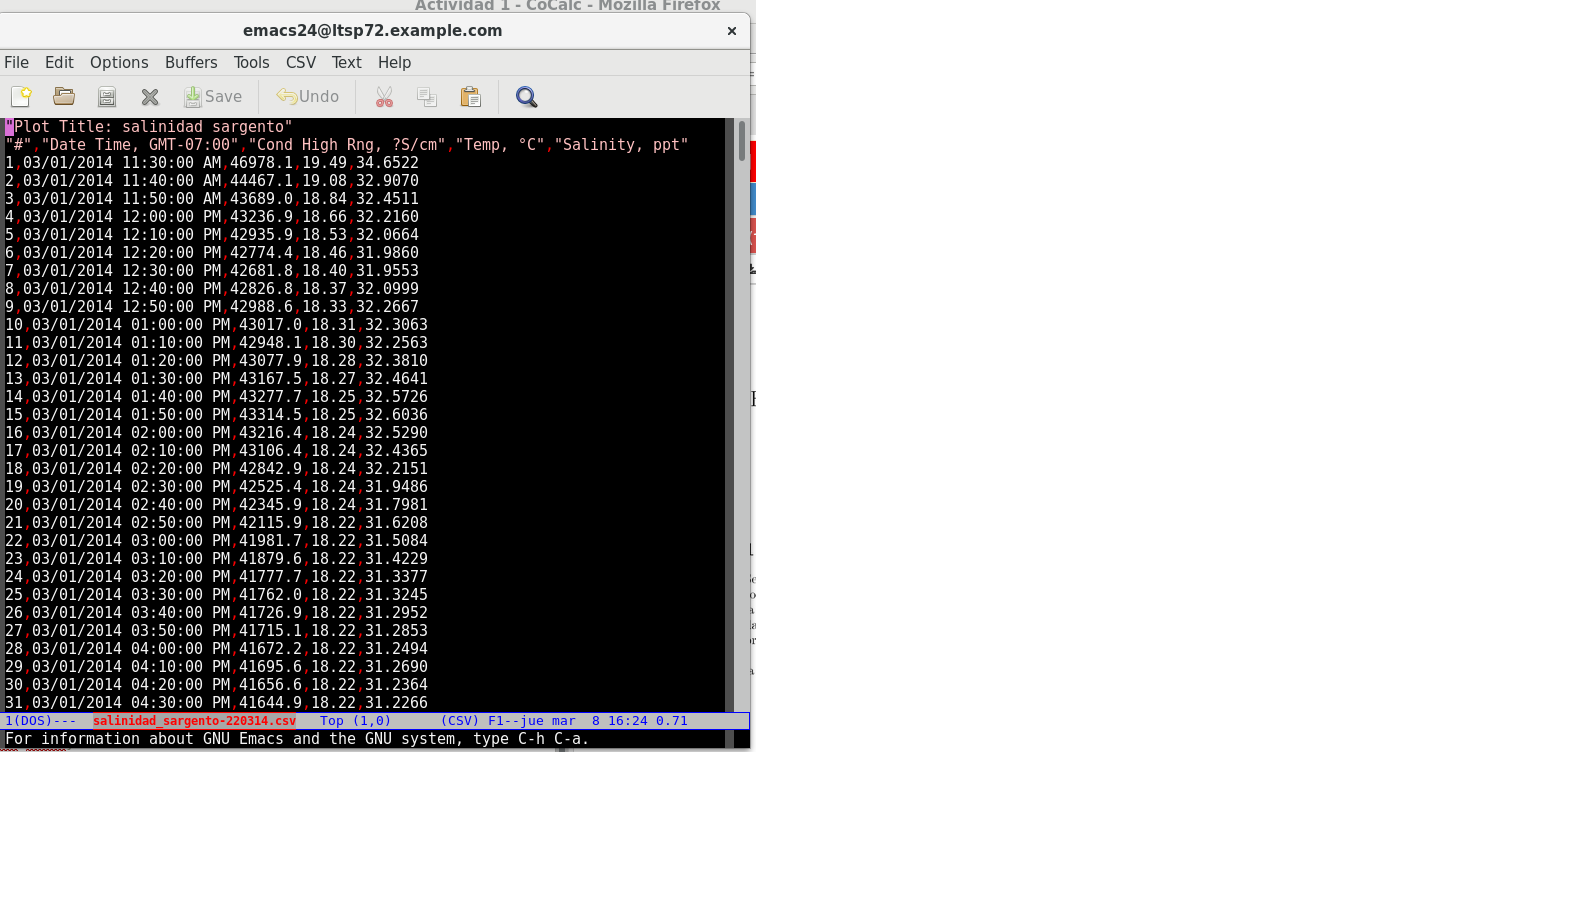
\includegraphics [width=20cm]{EstructuraDeDatos.png}
\centering
\caption{Así se ven los datos en el archivo abierto en \textit{emacs}}
\end{figure}

\subsection{Utilizar \textit{Python} y sus bibliotecas.}
Lo siguiente que hicimos fue cargar las bibliotecas que utilizaríamos para realizar todas las gráficas que nos pide.

\begin{figure}[H]
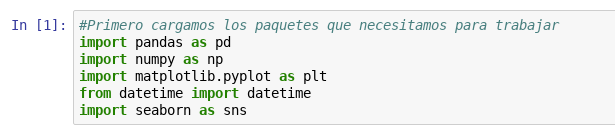
\includegraphics[width=\linewidth]{Import.png}
\caption{Estas son las bibliotecas necesarias para trabajar esta actividad}
\centering
\end{figure}
 
Algo que tuve que aprender a medio examen fue como combinar \textit{dataframes} en uno solo en \textit{Python}. 
Se utiliza un comando llamado \textit{concat} en el codigo de python y se procede a declarar todas las columnas de cada uno de los frames que queremos meter en el nuevo. el producto queda algo así:

\begin{figure}[H]
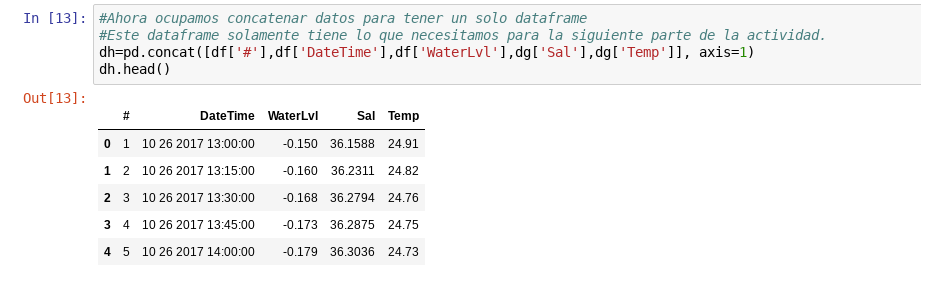
\includegraphics[width=\linewidth]{ConcatData.png}
\centering
\caption{Se juntan columnas de ambos archivos para su trabajo en un solo dataframe}
\end{figure}

\subsection{Talacha}
Una vez que tenemos el archivo limpio, las bibliotecas cargadas, y el dataframe unico, podemos proceder a dar la talacha que nos pide el profesor, cuyos resultados se presentan a continuación.

\section{Resultados}
\subsection{Graficas de Caja}

\begin{figure}[H]
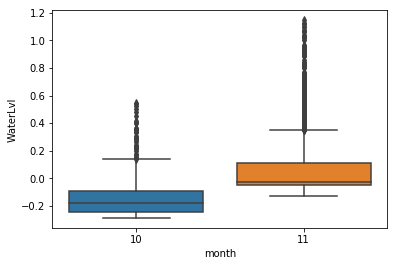
\includegraphics[width=\linewidth]{CajaH2O.png}
\centering
\caption{Grafica de caja del Nivel del Mar}
\end{figure}

\begin{figure}[H]
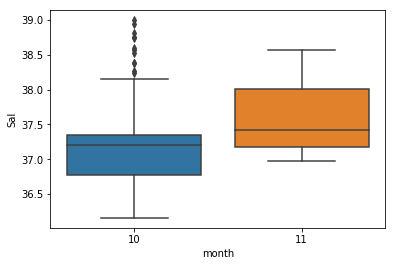
\includegraphics[width=\linewidth]{CajaSal.png}
\centering
\caption{Grafica de caja de Salinidad}
\end{figure}

\begin{figure}[H]
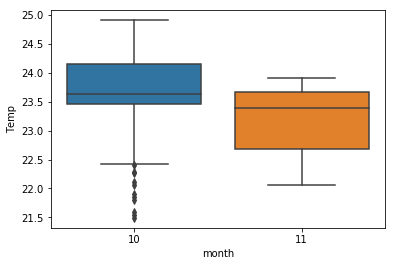
\includegraphics[width=\linewidth]{CajaTemp.png}
\centering
\caption{Grafica de Caja de la Temperatura}
\end{figure}

Como se puede ver, los datos estan tomados en dos meses diferentes, Octubre y Noviembre respectivamente.
\newline
De la misma manera se nos pidió que usaramos un \textit{dh.describe()} para los \textit{DataFrames}

\begin{figure}[H]
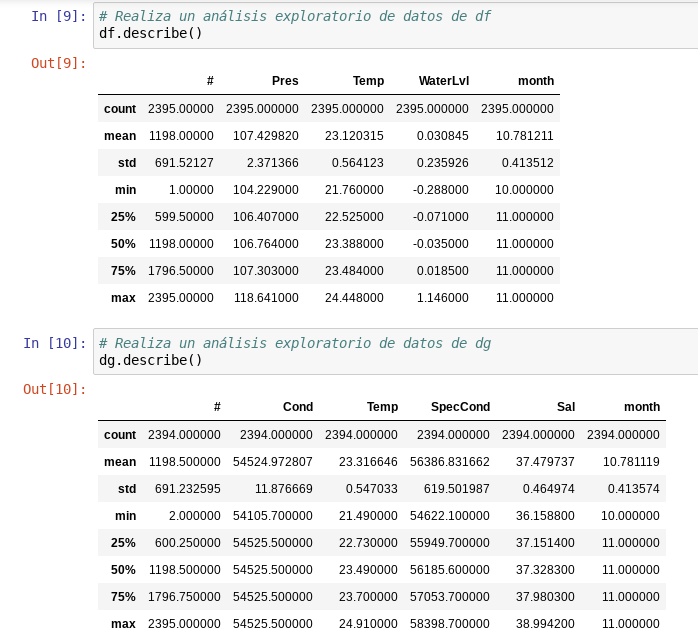
\includegraphics[width=\linewidth]{Descripcion.png}
\centering
\caption{}
\end{figure}

\subsection{Graficas de Regresión}
Se nos pidió sacar gráficas de regresión para observar la correlación entre distintas variables.

\begin{figure}[H]
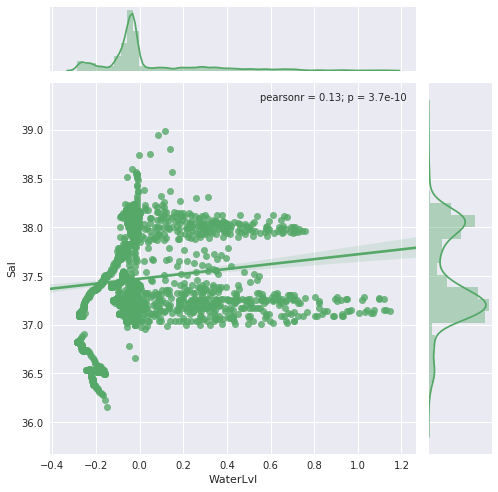
\includegraphics[width=\linewidth]{RegAguaSal.png}
\centering
\caption{Regresión de las variables Nivel del Mar y Salinidad}
\end{figure}

\begin{figure}[H]
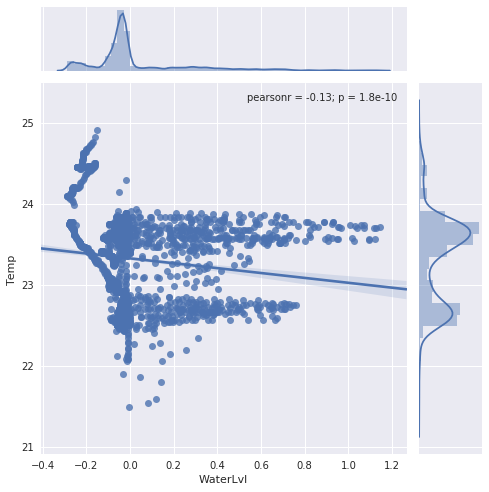
\includegraphics[width=\linewidth]{RegAguaTemp.png}
\centering
\caption{Regresión de las variables Nivel del Mar y Temperatura}
\end{figure}

\begin{figure}[H]
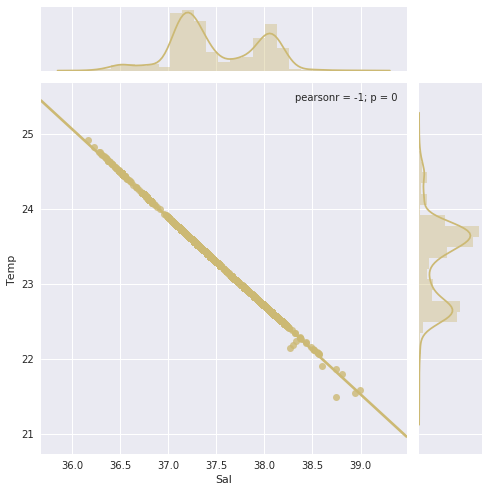
\includegraphics[width=\linewidth]{RegSalTemp.png}
\centering
\caption{Regresión de las variables Salinidad y Temperatura}
\end{figure}

\subsection{Graficas con \textit{Matplotlib}}
\subsubsection{Individuales}
Estas graficas son de una variable indivudual contra fecha.

\begin{figure}[H]
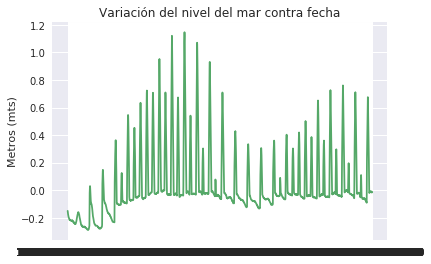
\includegraphics[width=\linewidth]{VarAguaFecha.png}
\centering
\caption{Variación del Nivel del Agua conforme pasa el tiempo}
\end{figure}

\begin{figure}[H]
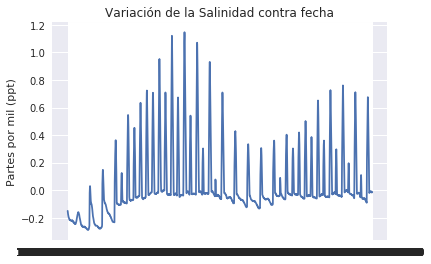
\includegraphics[width=\linewidth]{VarSalFecha.png}
\centering
\caption{Variación de la Salinidad conforme pasa el tiempo}
\end{figure}

\begin{figure}[H]
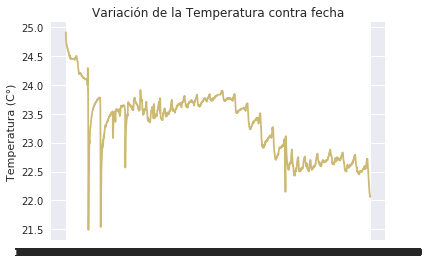
\includegraphics[width=\linewidth]{VarTempFecha.png}
\centering
\caption{Variación de la Temperatura conforme pasa el tiempo}
\end{figure}

\subsubsection{Dobles}
Estas gráficas se hicieron con eje Y doble, osease con dos variables para observar una relación con la fecha.

\begin{figure}[H]
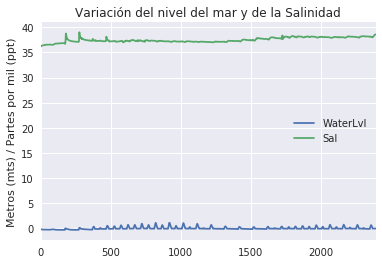
\includegraphics[width=\linewidth]{VarAguaSal.png}
\centering
\caption{Variación del Nivel del agua y de la Salinidad conforme pasa el tiempo}
\end{figure}

\begin{figure}[H]
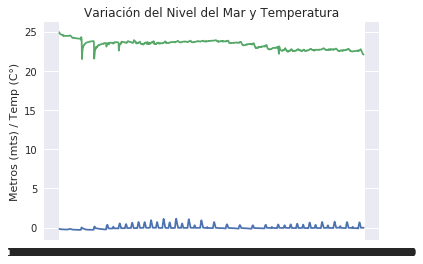
\includegraphics[width=\linewidth]{VarAguaTemp.png}
\centering
\caption{Variación del Nivel del agua y de la Temperatura conforme pasa el tiempo}
\end{figure}

\subsubsection{Dobles Acotadas}
Quizá el anterior tenía tantos datos que no se apreciaba tan bien una relación, esta vez actamos el frame a los utlimos 5 días de información recopilada con un comando \textit{Xlim} que limita el rango de la variable que está en el eje X, en este caso, la fecha.

\begin{figure}[H]
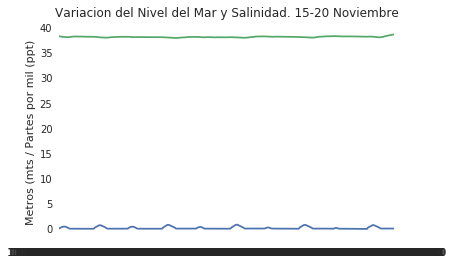
\includegraphics[width=\linewidth]{VarAguaSal_XLim.png}
\centering
\caption{Variación de Nivel del Agua y Salinidad del 15 al 20 de Noviembre del 2017}
\end{figure}

\begin{figure}[H]
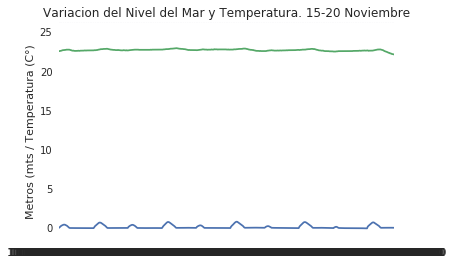
\includegraphics[width=\linewidth]{VarAguaTemp_XLim.png}
\centering
\caption{Variación del nivel del Agua y temperatura del 15 al 20 de noviembre del 2017}
\end{figure}

\section{Conclusiones}
Como podemos observar conforme a las graficas presentadas, podemos decir que la Salinidad tiene que ver con la temperatura del agua, ya que si la sal en el agua aumenta, inversamente lo hará la temperatura.
Tambien podemos decir claramente que el nivel del agua y la salinidad se encuentran relacionadas, sin embargo, estas también tienen que ver con las fechas, ya que, como sabemos, el nivel del mar es afectado por la gravitación de la luna y del Sol, pero si aumenta el nivel, también aumenta la cantidad de sal, puesto que trae más minerales de Sodio desde aguas mas profundas. Y la Temperatura pues depende mucho de la fecha, debido al calentamiento del agua debido al Sol.

\newpage

\section{Bibliografía}
\begin{itemize}
\item{Merge, Join and Concatenate, Revisado el 8 de Marzo del 2018} $https://pandas.pydata.org/pandas-docs/stable/merging.html$ 

\item{Pagina de Fisica Computacional 2018-1/Evaluación 1, Revisado el 8 de Marzo del 2018} 
$http://fisicacomputacional.pbworks.com/w/page/124361787/Evaluacion 1 (2018-1)$
\end{itemize}

\end{document}
